
% Lecture 3 - Syllabus, outline of class & intro to bayes
\documentclass[handout]{beamer}
\usepackage{pgfpages}
%\documentclass{beamer}
%\usepackage{beamerthemesplit}

\def\ce#1{\centerline{#1}}
\def\no{\noindent} 
\def\nl{\newline}
% -------
 \def\cblack{\color{black}}
 \def\cb{\color{blue}}
 \def\cred{\color{red}}
 \def\cy{\color{yellow}}
 \def\cg{\color{cyan}}
% -------
 \def\bs{\end{slide}\begin{slide}}
 \def\bi{\begin{itemize}} 
 \def\ei{\end{itemize}}
 \def\i{\item} 
 
\def\t{\theta} 
\def\l{\lambda} 
\def\d{\delta} 

\def\Pois{\mbox{Pois}} 
\def\Poisson{\mbox{Poisson}} 
\def\Exp{\mbox{Exp}} 
\def\Ga{\mbox{Ga}}
\def\Unif{\mbox{Unif}}
\def\Binomial{\mbox{Binomial}}
\def\Bernoulli{\mbox{Bernoulli}}

\def\Pr{\mbox{Pr}}
\def\E{\mbox{E}}
\def\Var{\mbox{V}}
\def\ind{\stackrel{ind}{\sim}}
\def\iid{\stackrel{iid}{\sim}}
\def\eps{\varepsilon}
\def\R{\mathbb{R}}
\def\Y{\mathcal{Y}}
\def\I{\mathcal{I}}
\def\PP{\mbox{PP}}



\title{STA 360/601: Bayesian and Modern Statistics}

\subtitle{Lecture 4: Poisson processes \& Non-informative priors}

\author{Jeff Miller}

\institute{Department of Statistical Science, Duke University}

\date{Friday, September 5, 2014}

\graphicspath{{figures/}}

\begin{document}

\frame{\titlepage}

%\section[Outline]{}
%\frame{\tableofcontents}

\section{Poisson process}

\frame{ \frametitle{Event time/location data}
    \begin{itemize}[<+-| alert@+>]
        \item Last lecture, we had count data $y_1,\ldots,y_n$, modeled as iid $\Poisson(\t)$.

        \item The Poisson likelihood also arises naturally when the data consist of timing or location of events.

        \item \underline{Examples}:
            \begin{itemize}
                \item $y_i$ = time of the $i$th traffic accident occurring at an intersection during 
                    the study period.

                \item $y_i$ = location of a microglia cell in a 3d brain image at snapshot in time.

                \item $y_i$ = time and location of a meteorite strike in the United States.
            \end{itemize}

        \item Often, a Poisson process is a natural model for such data.
    \end{itemize}
}

\frame{ \frametitle{}
1d example
\centerline{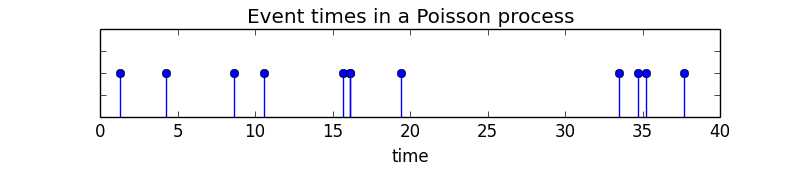
\includegraphics[width=8cm]{poisson1dt.png}}
\centerline{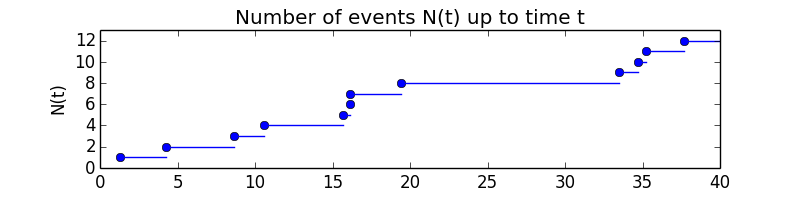
\includegraphics[width=8cm]{poisson1dN.png}}

2d example
\centerline{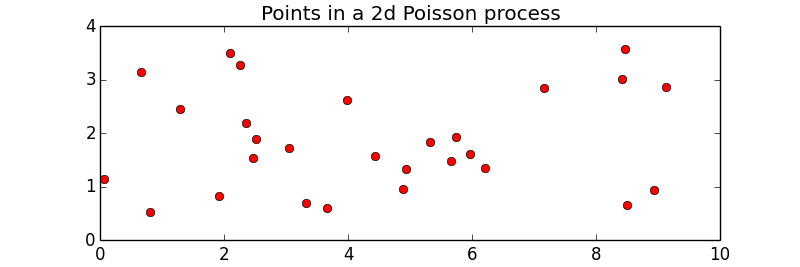
\includegraphics[width=8cm]{poisson2d.png}}
}

\frame{ \frametitle{Intuition for Poisson process}
    \begin{itemize}[<+-| alert@+>]
        \item Remember how $\Poisson(\t)$ is the limit of $\Binomial(n,\t/n)$ as $n\to\infty$?
        \item Think about that as dividing $[0,1]$ into $n$ intervals of length $1/n$ and putting a $\Bernoulli(\t/n)$ in each independently.
        \item Intuitively speaking, in terms of the Bernoullis (rather than their sum), the limiting thing you get is a Poisson process.
    \end{itemize}
}


\frame{ \frametitle{Poisson process on $[0,1]$}
    \begin{itemize}[<+-| alert@+>]
        \item A random set of points $\{Y_1,\ldots,Y_N\}\subset[0,1]$ are the points in a Poisson process on $[0,1]$ with rate $\t>0$ if 
              $N\sim\Poisson(\t)$ and $Y_1,\ldots,Y_N\iid \Unif(0,1)$ given $N$.
        \item Another useful construction (generates the points in order): $X_1,X_2,\ldots\iid \Exp(\t)$ and $Y_i=\sum_{j=1}^i X_j$ for
            $i=1,2,\ldots$ until $Y_i$ is no longer in $[0,1]$.
        \item Denote by $N(s,t)$ the \# of points $Y_i$ occurring in interval $(s,t]$. 
              For any $0\leq t_1<t_2<\cdots<t_k\leq 1$, $N(t_i,t_{i+1}) \ind \Poisson((t_{i+1}-t_i)\t)$ for $i=1,\ldots,k-1$.
        \item There are many equivalent formulations.
    \end{itemize}
}

%\frame{ \frametitle{Poisson process (1d, homogeneous)}
%Denote by $N(s,t)$ the \# of points occurring in interval $(s,t]$. \\
%The following are equivalent:
    %\begin{itemize}[<+-| alert@+>]
        %\item $Y_1,Y_2,\ldots$ are the points in a Poisson process on $[0,\infty)$ with rate $\t$.
        %\item $X_1,X_2,\ldots\iid \Exp(\t)$ and $Y_i=\sum_{j=1}^i X_j$.
        %\item If $0\leq t_1<t_2<\cdots<t_k$ then $N(t_i,t_{i+1}) \ind \Poisson((t_{i+1}-t_i)\t)$ for $i=1,\ldots,k-1$.
        %\item (a) Disjoint intervals have independent numbers of points, \\
            %(b) the distribution of $N(s,t)$ depends only on $t-s$, \\
            %(c) $\Pr(N(0,\eps)=1)/\eps \to \t$ as $\eps\to 0$, and \\
            %(d) $\Pr(N(0,\eps)\geq 2)/\eps \to 0$ as $\eps\to 0$. 
    %\end{itemize}
%}

\frame{ \frametitle{Thought experiment}
    \begin{itemize}[<+-| alert@+>]
        \item Let's think bigger\dots Why stop at $[0,1]$? Why not divide up $[0,\infty)$ into tiny intervals and do the same thing?
        \item Better yet: What if we took all of $\R^d$, divided it up into tiny boxes, and put an independent $\Bernoulli(p)$ in each,
            where $p$ is $\t$ times the volume of the box?
        \item Now we're getting somewhere\dots  But why limit ourselves to making every box have the same $p$?
        \item Let's take a function $r(y)\geq 0$ and define each $p$ as the integral of $r(y)$ over that box.
        \item This is the intuition behind the multidimensional inhomogeneous Poisson process.
    \end{itemize}
}

\frame{ \frametitle{Example}
    A sample from an inhomogeneous Poisson process on $\R^2$ with rate function $r(y) = \frac{1}{2}(\cos(\|y\|)+1).$
    \centerline{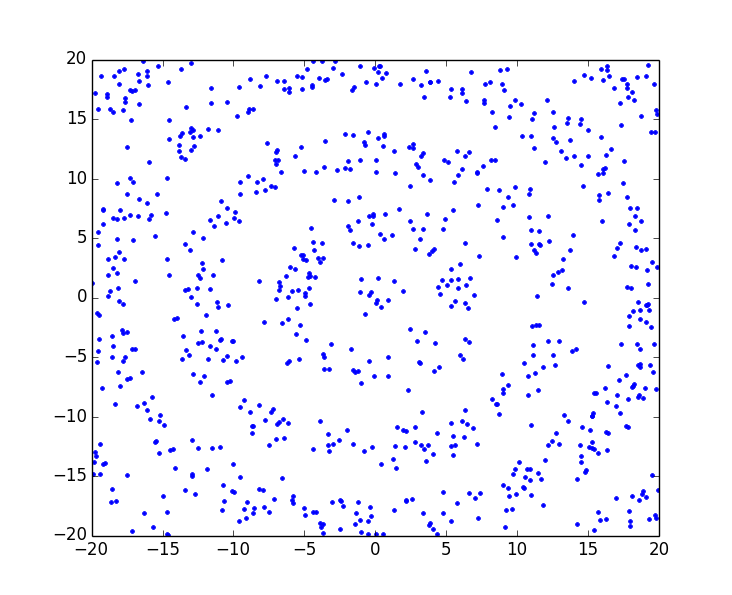
\includegraphics[width=9cm]{inhomog.png}}
}

\frame{ \frametitle{Poisson process (multidimensional, inhomogeneous)}
    \begin{itemize}[<+-| alert@+>]
        \item Assume $\int_A r(y)dy<\infty$ for $A\subset\R^d$ bounded.
        \item A Poisson process on $\R^d$ with rate function $r(y)\geq 0$ is a random countable set of points such that:\\
            \begin{enumerate}
                \item[(a)]  for any $A\subset\R^d$ the number of points $N(A)$ in $A$ is $\Poisson(\int_A r(y)dy)$, and \\
                \item[(b)]  $N(A_1),\ldots,N(A_k)$ are independent whenever $A_1,\ldots,A_k\subset\R^d$ are disjoint.
            \end{enumerate}
        \item Cool fact: When $c_r=\int_{\R^d} r(y)dy$ is finite, you can sample from a Poisson process by drawing $N\sim\Poisson(c_r)$ and
            then drawing the points $Y_1,\ldots,Y_N$ iid from the pdf $r(y)/c_r$.
        \item This last property allows us to write down the likelihood:
            $$L(y_{1:n};r) = \Pois(n;c_r) \prod_{i=1}^n r(y_i)/c_r.$$
    \end{itemize}
}

\frame{ \frametitle{Poisson process (homogeneous)}
    \begin{itemize}[<+-| alert@+>]
        \item Let's specialize to the homogeneous case, where $r(y)$ equals a constant $\t$ on a set $\Y$ of finite volume $v=\int_\Y dy$,
            and is $0$ elsewhere.
        \item Then $c_r=\t v$ and for $y_i\in\Y$, the likelihood simplifies to
            $$L(y_{1:n};\t) = \Pois(n;\t v) / v^n.$$
        \item The likelihood doesn't care about the locations of the points in $\Y$ --- only the number of points matters!
        \item So, once we choose a prior $\pi(\t)$ on $\t$, the posterior is just
            $$\pi(\t|y_{1:n}) \propto \Pois(n;\t v)\pi(\t).$$
    \end{itemize}
}

\frame{ \frametitle{Applications of Poisson processes}
    \begin{itemize}[<+-| alert@+>]
        \item The ``limit of Bernoulli processes'' perspective gives intuition into when a Poisson process model might be reasonable.
        \item Some more examples:
        \begin{itemize}
            \item times of neuron spikes,
            \item locations of mutations in a genome,
            \item times of speciation events in phylogenetic history,
            \item emission times of radioactively decaying particles,
            \item locations of organisms in a habitat at a given time.
        \end{itemize}
    \end{itemize}
}

\frame{ \frametitle{Illustration}
    \begin{itemize}[<+-| alert@+>]
        \item Patient A had $n=8$ seizures on the following days over the past $v=365$ days, with today as time 0:
            $$y=y_{1:n} = (-349, -297, -289, -251, -249, -202, -81, -69).$$
        \item A homogeneous Poisson process is a reasonable model (but probably too simplistic in reality).
        \item Based on a history of many previous patients, you have a prior $\pi(\t)$ on the rate.
        \item A certain treatment is known to be fully effective at preventing seizures ($E=1$) or have no effect ($E=0$), independently
            of $\t$ and $y$, with $\Pr(E=1) = q = 0.25$.
        \item Patient A is given the treatment today (time 0).
        \item $60$ days pass with no seizures. What is the probability that the treatment was effective?
    \end{itemize}
}


\frame{ \frametitle{Model}
    \begin{itemize}[<+-| alert@+>]
        \item[] $\t\sim \Ga(a,b)$ with $a=0.1$, $b=0.3$.
        \item[] $Y=Y_{1:N}\sim\PP(\t)$ on $[-365,0]$ given $\t$.
        \item[] $E\sim\Bernoulli(q)$ independent of $\t$ and $Y$.
        \item[] Given $\t,Y,E$, model future seizure times $Z_1\leq Z_2 \leq \cdots$ as a PP on $(0,\infty)$ with rate $0$ if effective
            ($E=1$) and rate $\t$ if not effective ($E=0$).
    \end{itemize}
}

\frame{ \frametitle{Quantity of interest}
    Probability of ineffective treatment, given no seizures up to $t$
    $$= \Pr(E=0\mid Z_1>t, y) = \frac{\Pr(Z_1>t\mid E=0,y)\Pr(E=0\mid y)}{\Pr(Z_1>t\mid y)}.$$
    We have $\Pr(E=0\mid y) = \Pr(E=0) = 1-q$ and
        \begin{align*}
            \Pr(Z_1>t\mid E=0,y) &= \int \Pr(Z_1>t\mid\t,E=0,y)\pi(\t\mid E=0,y)d\t \\
                                 &= \int \Pr(\Exp(\t)>t)\pi(\t|y)d\t \\
                                 &= \int e^{-\t t} \pi(\t|y)d\t,
        \end{align*}
        where the second step uses the fact that the time to the first event is $\Exp(\t)$ distributed (given $\t$ and $E=0$).
}

\frame{ \frametitle{Quantity of interest (continued)}
    The posterior on $\t$ given $y$ is (a lot like your last homework)
    $$\pi(\t|y_{1:n}) \propto \Pois(n;\t v)\Ga(\t;a,b) \propto \Ga(\t;a+n,b+v), $$
    so
    \begin{align*}
        \Pr(Z_1>t\mid E=0,y) &= \int_0^\infty e^{-\t t} \frac{(b+v)^{a+n}}{\Gamma(a+n)}\t^{a+n-1}e^{-(b+v)\t}d\t\\
                             &= \frac{(b+v)^{a+n}}{(b+v+t)^{a+n}},
    \end{align*}
    and thus, plugging this into the first equation of the previous slide,
    $$\Pr(E=0 \mid Z_1>t,y) = \frac{\big(\frac{b+v}{b+v+t}\big)^{a+n} (1-q)}{\Pr(Z_1>t\mid y)}.$$
}

\frame{ \frametitle{Quantity of interest (part trois)}
    Since $\Pr(E=1\mid Z_1>t,y) = q/\Pr(Z_1>t\mid y)$, and these two have to sum to $1$,
    %$\Pr(E=0\mid Z_1>t,y) + \Pr(E=1\mid Z_1>t,y)=1$, 
    we get
    $$\Pr(E=1 \mid Z_1>t,y) = \frac{q}{q+\big(\frac{b+v}{b+v+t}\big)^{a+n}(1-q)}.$$

    \centerline{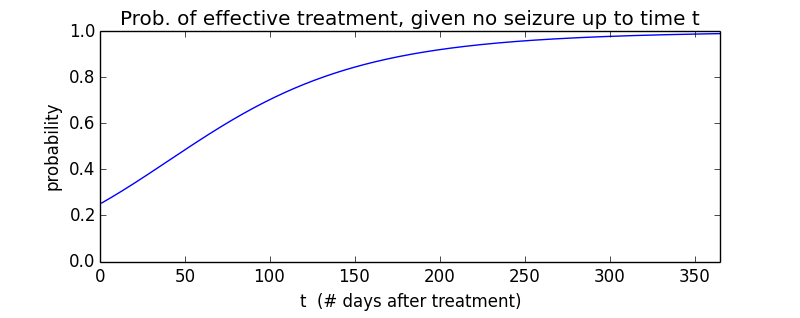
\includegraphics[width=10cm]{seizure.png}}
}

\frame{ \frametitle{A couple points}
    \begin{itemize}[<+-| alert@+>]
        \item Just applying the rules of probability, we can use the posterior to answer pretty much any reasonable question, e.g.:
        \begin{itemize}[<+-| alert@+>]
            \item Probability of seizure in next week, given no seizure up to now?
            \item If the treatment turns out to be ineffective, mean time to first seizure?
            \item One-sided prediction interval for time of first seizure?
            \item Patient wants to travel for 2 weeks where there are limited medical facilities;
                s/he could consider a loss function and make a decision.
        \end{itemize}
        %\item If we had side information about the patient that was informative about the probability of effective treatment, in principle
            %we could include that in the model, but inference might be harder.
        \item Due to homogeneity, our analysis only used $n$, not the values $y_1,\ldots,y_n$.
    \end{itemize}
}




\section{Non-informative priors}

\frame{ \frametitle{Objective Bayesian inference}
\begin{itemize}[<+-| alert@+>]
    \item If there is universally-accepted prior information, almost no one would argue with using it.
    \item But what if you really have no idea at all?
    \item Or, more likely, what if it is critical that your results not depend on any personal biases? e.g.,
    \begin{itemize}[<+-| alert@+>]
        \item clinical trials for a new drug,
        \item testing of a medical device,
        \item evidence to be presented in a court of law.
    \end{itemize}
    \item The original motivation of \emph{objective Bayes} was to find priors that contain little, or ideally, no information.
    \item That has evolved into a more attainable goal of finding ``default'' priors that provide reliable and interpretable results, to
        be used as conventions when more specific prior information can't or shouldn't be used.
\end{itemize}
}

 \frame{ \frametitle{Non-informative priors}
\begin{itemize}[<+-| alert@+>]
    \item Such priors $\pi(\t)$ are called \emph{non-informative}, and they are usually \emph{improper}, in the sense that they do not
        integrate to a finite value, i.e., $\int \pi(\t)d\t = \infty$.

    \item For example, suppose we choose a gamma prior $\theta \sim \mbox{Ga}(a,b)$.

    \item Then, since the prior variance $\Var(\theta) = a/b^2$ is finite, in some sense the prior contains some information.

    \item This is apparent in the {\em shrinkage} that occurs, with the posterior mean being a convex combination of the sample mean and prior mean.

    \item If we take $a=b=\eps$ for $\eps$ small, the prior mean stays at $a/b=1$ and the variance becomes large.
        As $\eps\to 0$, the shape of the prior becomes $\propto 1/\theta$.

    \item This is one example of an improper prior.
\end{itemize}
}

 \frame{ \frametitle{Improper priors}
\begin{itemize}[<+-| alert@+>]
\item Improper priors are in some sense not priors at all in that they aren't probability densities.

\item There is no prior mean or defined prior variance, we can't sample from an improper prior, 
    and the prior predictive $p(y)=\int p(y|\t)\pi(\t)d\t$ is undefined.

\item However, motivated by a desire to avoid having information in our prior, we can plug an improper prior into Bayes' rule.

\item In many cases, the resulting ``posterior'' (defined in a formal sense via Bayes' rule) is a proper density.

\item Bayesian inferences can be conducted \underline{only if} the resulting posterior is proper.
\end{itemize}
}

\frame{ \frametitle{Illustration}
Suppose we use $\pi(\t)=1/\t$ in our seizure example. Formally,
\begin{align*}
    \pi(\t|y) &\propto \mbox{likelihood}\times\mbox{prior} = \Pois(n;\t v)\pi(\t) \\
    &=e^{-\t v}\frac{(\t v)^n}{n!}\frac{1}{\t} \propto \t^{n-1}e^{-v \t} \\
    & \propto \Ga(\t; n,v).
\end{align*}
So it's like setting $a=b=0$ in our posterior from before.
%Plugging this in, we get 
    %$$\Pr(E=1 \mid Z_1>t,y) = \frac{q}{q+\big(\frac{v}{v+t}\big)^n(1-q)}.$$
How does it compare to the result with our proper prior?
\centerline{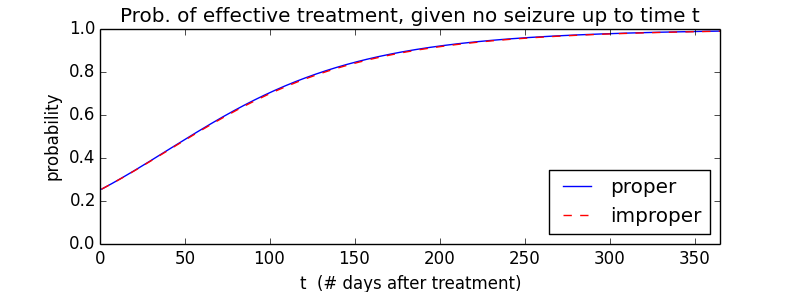
\includegraphics[width=8cm]{improper.png}}

In this case, they are nearly identical.
}

%\frame{ \frametitle{Some ways of constructing non-informative priors}
    %\begin{itemize}[<+-| alert@+>]
        %\item ...
    %\end{itemize}
%}

\frame{ \frametitle{Comments on improper priors}
\begin{itemize}[<+-| alert@+>]
    \item Never use them unless you are sure the resulting posterior is proper.

    \item If the posterior is improper, inferences are typically meaningless --- posterior mean, credible intervals, etc., are undefined.

    \item Even if the posterior is proper, serious issues can arise: contradictory probabilities, prior can dominate for large $n$,
        inadmissible estimators, marginalization paradoxes.

\end{itemize}
}

 
\frame{ \frametitle{Comments on improper priors (continued)}
\begin{itemize}[<+-| alert@+>]
    \item Bayesian inferences under improper priors are sometimes more similar to frequentist inferences.

    %\item However, the Bayesian paradigm is still used to characterize uncertainty.

    \item In many (most?) situations a weakly informative prior will outperform a non-informative one.

    \item In small sample sizes and data sparse situations, weakly informative 
    priors stabilize inferences through mild shrinkage towards the prior mean.

    \item The age old bias-variance tradeoff --- the prior introduces a bit of bias to greatly reduce variance.
\end{itemize}
}


\frame{ \frametitle{Homework exercise}
\begin{itemize}[<+-| alert@+>]
    \item The Jeffreys prior is a classical non-informative prior, defined (for a univariate parameter) as
        $\pi(\t) \propto \sqrt{\I(\t)}$ where
        $$ \I(\t) = \int\Big(\frac{\partial}{\partial\t}\log p(y|\t)\Big)^2 p(y|\t)dy$$
        is the \emph{Fisher information}.
    \item Show that for any likelihood $p(y|\t)$, if $\pi(\t)$ is the Jeffreys prior, and 
        we have an alternate parametrization, say $q(y|\phi)=p(y|\t)$ where $\t=h(\phi)$ and $h$ is a
        smooth 1-to-1 function, then the Jeffreys prior $\bar\pi(\phi)$ for $\phi$ satisfies
        $$\bar\pi(\phi) \propto \pi(h(\phi))|h'(\phi)|.$$
        (Hint: Let $\ell(\t)=\log p(y|\t)$ and apply the chain rule to compute $\frac{\partial}{\partial\phi} \ell(h(\phi))$.)
    \item Explain why this property is appealing.
    %\item Compute the Jeffreys prior for the Poisson likelihood $p(y|\t) = e^{-\t} \t^y / y!$.
        %and verify this invariance directly for the reparametrization $\phi = \log(\t)$.
\end{itemize}
}


\frame{ \frametitle{References}
    Poisson processes
    \begin{itemize}[<+-| alert@+>]
        \item Grimmett \& Stirzaker, \emph{Probability and Random Processes}, Oxford University Press, 2006. (Secs 6.8, 6.13)
        \item Rick Durrett, \emph{Probability: Theory and Examples}, Duxbury Press, 1996. (pp. 145--148)
    \end{itemize}

    Non-informative priors
    \begin{itemize}[<+-| alert@+>]
        \item Kass \& Wasserman, \emph{The selection of prior distributions by formal rules}, JASA, Vol.\ 91, No.\ 435, 1996.
        \item James O.\ Berger, \emph{Statistical Decision Theory and Bayesian Analysis}, Springer-Verlag, 1985. (Sec 3.3)
    \end{itemize}
}




\end{document} 







